\documentclass{beamer}
\usetheme{Boadilla}
\setbeamertemplate{navigation symbols}{}

\usepackage{booktabs}
\usepackage{pgf-umlcd}
\usepackage{pgf}
\usepackage{tikz}
% Pointed set
\newcommand{\pset}[2]{\ensuremath{\left(#1,\,#2\right)}}

% Maps
\newcommand{\keyset}{\ensuremath{\mathrm{K}}}
\newcommand{\valset}{\ensuremath{\mathrm{V}}}
\newcommand{\map}[2]{\ensuremath{\mathrm{Map}\ #1\;#2}}
\newcommand{\finitemap}[2]{\ensuremath{\mathrm{Map}_*\ #1\;#2}}
\input{code/lhs2tex.tex}

\title[JOINBENCH]{JOINBENCH: Designing Tools for the Evaluation of Efficient Equijoins in Haskell}
\author[Matteo Bongiovanni]{Matteo Bongiovanni\\\vspace{4mm}{\scriptsize Supervisor: Dr. Nicolas
Wu\hspace{4mm}Second Marker: Dr. Steffen van Bakel}}
\date[]{MEng Individual Project, 31 August 2023}
\institute[JMC]{Joint Mathematics and Computing \\ Department of Computing}
\titlegraphic{\includegraphics[height=1cm]{title/logo.eps}}

\begin{document}
\frame{\titlepage}

\begin{frame}
\frametitle{Introduction}
\end{frame}

\begin{frame}
\frametitle{Presentation Outline}
\tableofcontents
\end{frame}

\section{Database Implementation}
\begin{frame}
\frametitle{Bags -- Definition and Equality}
\begin{hscode}\SaveRestoreHook
\column{B}{@{}>{\hspre}l<{\hspost}@{}}%
\column{5}{@{}>{\hspre}l<{\hspost}@{}}%
\column{7}{@{}>{\hspre}l<{\hspost}@{}}%
\column{9}{@{}>{\hspre}l<{\hspost}@{}}%
\column{11}{@{}>{\hspre}l<{\hspost}@{}}%
\column{13}{@{}>{\hspre}l<{\hspost}@{}}%
\column{17}{@{}>{\hspre}l<{\hspost}@{}}%
\column{26}{@{}>{\hspre}c<{\hspost}@{}}%
\column{26E}{@{}l@{}}%
\column{29}{@{}>{\hspre}l<{\hspost}@{}}%
\column{E}{@{}>{\hspre}l<{\hspost}@{}}%
\>[B]{}\mathbf{newtype}\;\Conid{Bag}\;\Varid{a}\mathrel{=}\Conid{Bag}\;\{\mskip1.5mu \Varid{elements}\mathbin{::}[\mskip1.5mu \Varid{a}\mskip1.5mu]\mskip1.5mu\}{}\<[E]%
\\[\blanklineskip]%
\>[B]{}\mathbf{instance}\;(\Conid{Eq}\;\Varid{a})\Rightarrow \Conid{Eq}\;(\Conid{Bag}\;\Varid{a})\;\mathbf{where}{}\<[E]%
\\
\>[B]{}\hsindent{5}{}\<[5]%
\>[5]{}\Varid{b1}\equiv \Varid{b2}\mathrel{=}\Varid{eq'}\;(\Varid{elements}\;\Varid{b1})\;(\Varid{elements}\;\Varid{b2}){}\<[E]%
\\
\>[5]{}\hsindent{2}{}\<[7]%
\>[7]{}\mathbf{where}{}\<[E]%
\\
\>[7]{}\hsindent{2}{}\<[9]%
\>[9]{}\Varid{eq'}\mathbin{::}{}\<[17]%
\>[17]{}(\Conid{Eq}\;\Varid{a})\Rightarrow [\mskip1.5mu \Varid{a}\mskip1.5mu]\to [\mskip1.5mu \Varid{a}\mskip1.5mu]\to \Conid{Bool}{}\<[E]%
\\
\>[7]{}\hsindent{2}{}\<[9]%
\>[9]{}\Varid{eq'}\;(\Varid{x}\mathbin{:}\Varid{xs})\;\Varid{ys}{}\<[26]%
\>[26]{}\mathrel{=}{}\<[26E]%
\>[29]{}\neg \;(\Varid{null}\;\Varid{ys2})\mathrel{\wedge}\Varid{eq'}\;\Varid{xs}\;(\Varid{ys1}\plus \Varid{tail}\;\Varid{ys2}){}\<[E]%
\\
\>[9]{}\hsindent{2}{}\<[11]%
\>[11]{}\mathbf{where}{}\<[E]%
\\
\>[11]{}\hsindent{2}{}\<[13]%
\>[13]{}(\Varid{ys1},\Varid{ys2})\mathrel{=}\Varid{break}\;(\equiv \Varid{x})\;\Varid{ys}{}\<[E]%
\\
\>[7]{}\hsindent{2}{}\<[9]%
\>[9]{}\Varid{eq'}\;[\mskip1.5mu \mskip1.5mu]\;[\mskip1.5mu \mskip1.5mu]{}\<[26]%
\>[26]{}\mathrel{=}{}\<[26E]%
\>[29]{}\Conid{True}{}\<[E]%
\\
\>[7]{}\hsindent{2}{}\<[9]%
\>[9]{}\Varid{eq'}\;\anonymous \;\anonymous {}\<[26]%
\>[26]{}\mathrel{=}{}\<[26E]%
\>[29]{}\Conid{False}{}\<[E]%
\ColumnHook
\end{hscode}\resethooks

\end{frame}
\begin{frame}
\frametitle{Bags -- Relational Algebra Operations}
\begin{table}[h]
    \centering
    \begin{tabular}{r|l}
        table of $V$ values & \bag{V} \\
        empty table & \emptybag \\
        singleton table & \singletonbag \\
        union of tables & $\bagunion{}{}$ \\
        Cartesian product of tables & $\times$ \\
        neutral element & $\lbag () \rbag$ \\
        projection $\projsymb{f}$ & $\bag{f}$ \\
        selection $\selectsymb{p}$ & $filter\ p$ \\
        aggregation in monoid $\monoid{M}$ & $reduce\ \monoid{M}$\\
    \end{tabular}
\end{table}
\end{frame}

\begin{frame}
\frametitle{Pointed sets, finite maps and indexed tables}
\begin{block}{Pointed set}
\end{block}
\begin{block}{Finite map}
\end{block}
\begin{block}{Indexed table}
\end{block}

\begin{table}[h]
    \centering
    \begin{tabular}{r|l}
        \keyset{}-indexed table of \valset{} values & \indexedTable{\keyset}{\valset} \\
        empty table & $empty$ \\
        singleton table $(k, v)$ & $k \mapsto \lbag v \rbag$ \\
        union of tables & $\finitemap{\keyset}{(\uplus)}\ \cdot\ merge$ \\
        projection $\projsymb{f}$ & $\finitemap{\keyset}{(\finitebag{f})}$ \\
        selection $\selectsymb{p}$ & $\finitemap{\keyset}{(filter\ p)}$ \\
        aggregation in monoid $\monoid{M}$ & $\finitemap{\keyset}{(reduce\
        \monoid{M})}$\\
            natural join & \finitemap{\keyset}{(\times)}\ $\cdot\ merge$ \\
    \end{tabular}
\end{table}
\end{frame}

\begin{frame}
    \frametitle{Indexed table implementation}
    \begin{hscode}\SaveRestoreHook
\column{B}{@{}>{\hspre}l<{\hspost}@{}}%
\column{5}{@{}>{\hspre}l<{\hspost}@{}}%
\column{7}{@{}>{\hspre}l<{\hspost}@{}}%
\column{9}{@{}>{\hspre}l<{\hspost}@{}}%
\column{27}{@{}>{\hspre}c<{\hspost}@{}}%
\column{27E}{@{}l@{}}%
\column{30}{@{}>{\hspre}l<{\hspost}@{}}%
\column{E}{@{}>{\hspre}l<{\hspost}@{}}%
\>[B]{}\mathbf{instance}\;\Conid{Key}\;\Conid{Word16}\;\mathbf{where}\;\mbox{\onelinecomment  constant type (array indexed by 16 bit word)}{}\<[E]%
\\
\>[B]{}\hsindent{5}{}\<[5]%
\>[5]{}\mathbf{newtype}\;\Conid{Map}\;\Conid{Word16}\;\Varid{v}{}\<[27]%
\>[27]{}\mathrel{=}{}\<[27E]%
\>[30]{}\Conid{A}\;(\Conid{Array}\;\Conid{Word16}\;\Varid{v})\;\mathbf{deriving}\;(\Conid{Eq},\Conid{Show}){}\<[E]%
\\
\>[B]{}\hsindent{5}{}\<[5]%
\>[5]{}\Varid{empty}{}\<[27]%
\>[27]{}\mathrel{=}{}\<[27E]%
\>[30]{}\Conid{A}\;(\Varid{accumArray}\;(\mathbin{\char92 \char95 }\Varid{x}\to \Varid{x})\;\Varid{\Conid{PointedSet}.null}\;(\mathrm{0},\mathrm{2}\mathbin{\uparrow}\mathrm{16}\mathbin{-}\mathrm{1})\;[\mskip1.5mu \mskip1.5mu]){}\<[E]%
\\
\>[B]{}\hsindent{5}{}\<[5]%
\>[5]{}\Varid{isEmpty}\;(\Conid{A}\;\Varid{a}){}\<[27]%
\>[27]{}\mathrel{=}{}\<[27E]%
\>[30]{}\Varid{all}\;\Varid{isNull}\;(\Varid{elems}\;\Varid{a}){}\<[E]%
\\
\>[B]{}\hsindent{5}{}\<[5]%
\>[5]{}\Varid{single}\;(\Varid{k},\Varid{v}){}\<[27]%
\>[27]{}\mathrel{=}{}\<[27E]%
\>[30]{}\Conid{A}\;(\Varid{accumArray}\;(\mathbin{\char92 \char95 }\Varid{x}\to \Varid{x})\;\Varid{\Conid{PointedSet}.null}\;(\mathrm{0},\mathrm{2}\mathbin{\uparrow}\mathrm{16}\mathbin{-}\mathrm{1})\;[\mskip1.5mu (\Varid{k},\Varid{v})\mskip1.5mu]){}\<[E]%
\\
\>[B]{}\hsindent{5}{}\<[5]%
\>[5]{}\Varid{merge}\;(\Conid{A}\;\Varid{a1},\Conid{A}\;\Varid{a2}){}\<[27]%
\>[27]{}\mathrel{=}{}\<[27E]%
\>[30]{}\Conid{A}\;(\Varid{listArray}\;(\mathrm{0},\mathrm{2}\mathbin{\uparrow}\mathrm{16}\mathbin{-}\mathrm{1})\;(\Varid{zip}\;(\Varid{elems}\;\Varid{a1})\;(\Varid{elems}\;\Varid{a2}))){}\<[E]%
\\
\>[B]{}\hsindent{5}{}\<[5]%
\>[5]{}\Varid{dom}\;(\Conid{A}\;\Varid{a}){}\<[27]%
\>[27]{}\mathrel{=}{}\<[27E]%
\>[30]{}\Conid{Bag}\;[\mskip1.5mu \Varid{k}\mid (\Varid{k},\Varid{v})\leftarrow \Varid{assocs}\;\Varid{a},\neg \;(\Varid{isNull}\;\Varid{v})\mskip1.5mu]{}\<[E]%
\\
\>[B]{}\hsindent{5}{}\<[5]%
\>[5]{}\Varid{cod}\;(\Conid{A}\;\Varid{a}){}\<[27]%
\>[27]{}\mathrel{=}{}\<[27E]%
\>[30]{}\Conid{Bag}\;[\mskip1.5mu \Varid{v}\mid (\Varid{k},\Varid{v})\leftarrow \Varid{assocs}\;\Varid{a},\neg \;(\Varid{isNull}\;\Varid{v})\mskip1.5mu]{}\<[E]%
\\
\>[B]{}\hsindent{5}{}\<[5]%
\>[5]{}\Varid{lookup}\;(\Conid{A}\;\Varid{a}){}\<[27]%
\>[27]{}\mathrel{=}{}\<[27E]%
\>[30]{}(\mathbin{!})\;\Varid{a}{}\<[E]%
\\
\>[B]{}\hsindent{5}{}\<[5]%
\>[5]{}\Varid{index}\;\Varid{kvps}{}\<[27]%
\>[27]{}\mathrel{=}{}\<[27E]%
\>[30]{}\Conid{A}\;(\Varid{accumArray}\;(\Varid{curry}\;\Varid{\Conid{Bag}.union})\;\Varid{\Conid{Bag}.empty}\;(\mathrm{0},\mathrm{2}\mathbin{\uparrow}\mathrm{16}\mathbin{-}\mathrm{1})\;\Varid{vals}){}\<[E]%
\\
\>[5]{}\hsindent{2}{}\<[7]%
\>[7]{}\mathbf{where}{}\<[E]%
\\
\>[7]{}\hsindent{2}{}\<[9]%
\>[9]{}\Varid{vals}{}\<[27]%
\>[27]{}\mathrel{=}{}\<[27E]%
\>[30]{}(\Varid{elements}\mathbin{\circ}\Varid{fmap}\;(\Varid{\Conid{Bifunctor}.second}\;\Varid{\Conid{Bag}.single}))\;\Varid{kvps}{}\<[E]%
\\
\>[B]{}\hsindent{5}{}\<[5]%
\>[5]{}\Varid{unindex}\;(\Conid{A}\;\Varid{a}){}\<[27]%
\>[27]{}\mathrel{=}{}\<[27E]%
\>[30]{}\Conid{Bag}\;[\mskip1.5mu (\Varid{k},\Varid{v})\mid (\Varid{k},\Varid{vs})\leftarrow \Varid{assocs}\;\Varid{a},\Varid{v}\leftarrow \Varid{elements}\;\Varid{vs}\mskip1.5mu]{}\<[E]%
\ColumnHook
\end{hscode}\resethooks

\end{frame}

\section{\relation{JOINBENCH} table}
\begin{frame}
\frametitle{The \relation{JOINBENCH} table}
\begin{table}
    \centering
    \begin{tabular}{ll}
        \toprule
        Attribute & Domain \\
        \midrule
        \relation{unique} & Int \\
        \relation{onePercent} & Word16 \\
        \relation{twentyPercent} & Word16 \\
        \relation{twentyFivePercent} & Word16 \\
        \relation{fiftyPercent} & Word16 \\
        \relation{evenOnePercent} & Word16 \\
        \relation{oddOnePercent} & Word16 \\
        \bottomrule
    \end{tabular}
\end{table}
\end{frame}

\section{Synthetic Database Generation}
\begin{frame}
\frametitle{Overview}
\begin{figure}
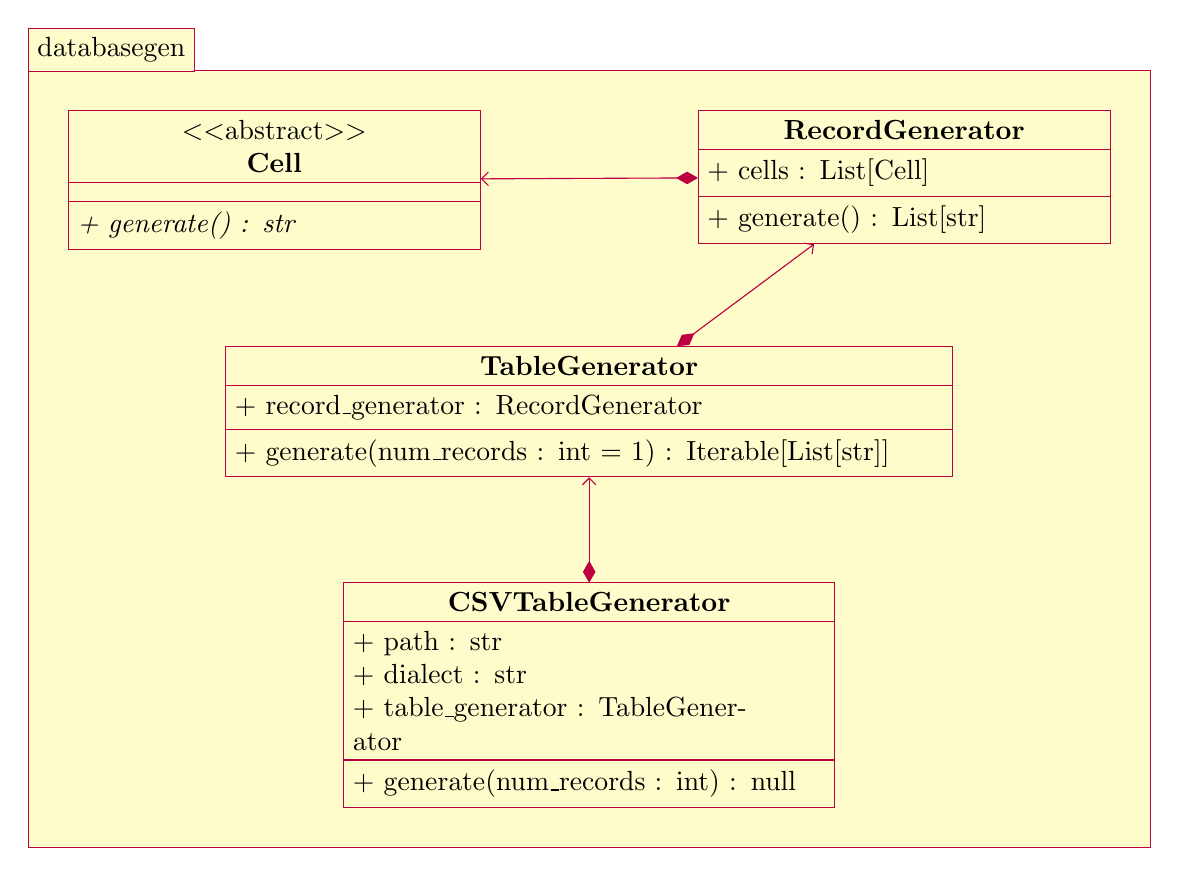
\begin{tikzpicture}
    \begin{package}{databasegen}
        \begin{abstractclass}{Cell}{-4,0}
            \operation[0]{+ generate() : str}
        \end{abstractclass}

        \begin{class}{RecordGenerator}{4, 0}
            \attribute{+ cells : List[Cell]}
            \operation{+ generate() : List[str]}
        \end{class}

        \begin{class}[text width=9cm]{TableGenerator}{0, -3}
            \attribute{+ record\_generator : RecordGenerator}
            \operation{+ generate(num\_records : int = 1) : Iterable[List[str]]}
        \end{class}

        \begin{class}[text width=6cm]{CSVTableGenerator}{0, -6}
            \attribute{+ path : str}
            \attribute{+ dialect : str}
            \attribute{+ table\_generator : TableGenerator}
            \operation{+ generate(num\_records : int) : null}
        \end{class}

        \composition{RecordGenerator}{}{}{Cell}
        \composition{TableGenerator}{}{}{RecordGenerator}
        \composition{CSVTableGenerator}{}{}{TableGenerator}
    \end{package}
\end{tikzpicture}
\end{figure}
\end{frame}

\begin{frame}
\frametitle{Cells}
\begin{itemize}
    \item Introduction
    \item Cell comprehension
    \item Integer cells
\begin{figure}[t]
    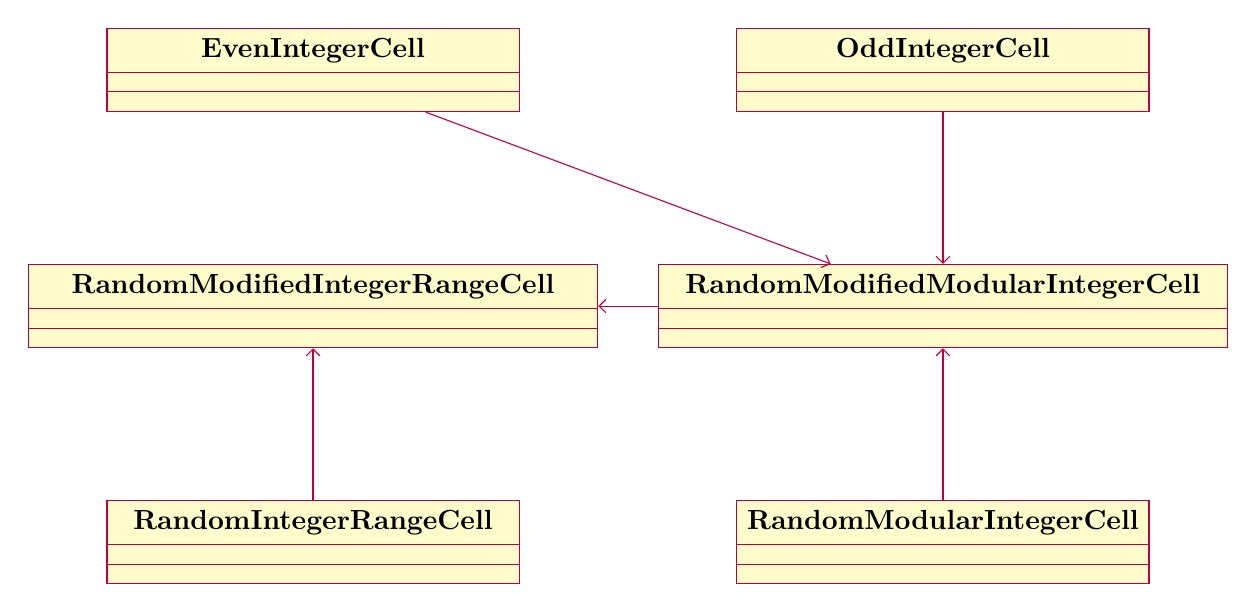
\begin{tikzpicture}
        \begin{class}{RandomIntegerRangeCell}{0, -3}
        \end{class}
        \begin{class}[text width=7cm]{RandomModifiedIntegerRangeCell}{0, -0}
        \end{class}
        \begin{class}{RandomModularIntegerCell}{8, -3}
        \end{class}
        \begin{class}[text width=7cm]{RandomModifiedModularIntegerCell}{8, -0}
        \end{class}
        \begin{class}{EvenIntegerCell}{0, 3}
        \end{class}
        \begin{class}{OddIntegerCell}{8, 3}
        \end{class}

        \unidirectionalAssociation{EvenIntegerCell}{}{}{RandomModifiedModularIntegerCell}
        \unidirectionalAssociation{OddIntegerCell}{}{}{RandomModifiedModularIntegerCell}
        \unidirectionalAssociation{RandomIntegerRangeCell}{}{}{RandomModifiedIntegerRangeCell}
        \unidirectionalAssociation{RandomModifiedModularIntegerCell}{}{}{RandomModifiedIntegerRangeCell}
        \unidirectionalAssociation{RandomModularIntegerCell}{}{}{RandomModifiedModularIntegerCell}
    \end{tikzpicture}
\end{figure}
\end{itemize}
\end{frame}

\section{Benchmarking}
\begin{frame}
\frametitle{Functions}
\begin{block}{Product equijoin}
    \vspace{-4mm}
    {\scriptsize\begin{hscode}\SaveRestoreHook
\column{B}{@{}>{\hspre}l<{\hspost}@{}}%
\column{3}{@{}>{\hspre}l<{\hspost}@{}}%
\column{5}{@{}>{\hspre}l<{\hspost}@{}}%
\column{E}{@{}>{\hspre}l<{\hspost}@{}}%
\>[B]{}\Varid{indexedEquijoin}\mathbin{::}(\Conid{Key}\;\Varid{k})\Rightarrow
(\Varid{a}\to \Varid{k})\to (\Varid{b}\to \Varid{k})\to
(\Conid{Bag}\;\Varid{a},\Conid{Bag}\;\Varid{b})\to \Conid{Bag}\;(\Varid{a},\Varid{b}){}\<[E]%
\\
\>[B]{}\Varid{indexedEquijoin}\;\Varid{if1}\;\Varid{if2}\;(\Varid{t1},\Varid{t2})\mathrel{=}(\Varid{reduce}\mathbin{\circ}\Varid{fmap}\;\Varid{cp}\mathbin{\circ}\Varid{merge})\;(\Varid{it1},\Varid{it2}){}\<[E]%
\\
\>[B]{}\hsindent{3}{}\<[3]%
\>[3]{}\mathbf{where}{}\<[E]%
\\
\>[3]{}\hsindent{2}{}\<[5]%
\>[5]{}\Varid{it1}\mathrel{=}\Varid{t1}\mathbin{`\Varid{indexBy}`}\Varid{if1}{}\<[E]%
\\
\>[3]{}\hsindent{2}{}\<[5]%
\>[5]{}\Varid{it2}\mathrel{=}\Varid{t2}\mathbin{`\Varid{indexBy}`}\Varid{if2}{}\<[E]%
\ColumnHook
\end{hscode}\resethooks
}
    \vspace{-7mm}
\end{block}\pause
\begin{block}{Comprehension equijoin}
    \vspace{-4mm}
    {\scriptsize\begin{hscode}\SaveRestoreHook
\column{B}{@{}>{\hspre}l<{\hspost}@{}}%
\column{E}{@{}>{\hspre}l<{\hspost}@{}}%
\>[B]{}\Varid{comprehensionEquijoin}\mathbin{::}(\Conid{Eq}\;\Varid{c})\Rightarrow
(\Varid{a}\to \Varid{c})\to (\Varid{b}\to \Varid{c})\to
(\Conid{Bag}\;\Varid{a},\Conid{Bag}\;\Varid{b})\to \Conid{Bag}\;(\Varid{a},\Varid{b}){}\<[E]%
\\
\>[B]{}\Varid{comprehensionEquijoin}\;\Varid{fa}\;\Varid{fb}\;(\Varid{as},\Varid{bs})\mathrel{=}[\mskip1.5mu (\Varid{a},\Varid{b})\mid \Varid{a}\leftarrow \Varid{as},\Varid{b}\leftarrow \Varid{bs},\Varid{fa}\;\Varid{a}\equiv \Varid{fb}\;\Varid{b}\mskip1.5mu]{}\<[E]%
\ColumnHook
\end{hscode}\resethooks
}
    \vspace{-7mm}
\end{block}\pause
\begin{block}{Indexed equijoin}
    \vspace{-4mm}
    {\scriptsize\begin{hscode}\SaveRestoreHook
\column{B}{@{}>{\hspre}l<{\hspost}@{}}%
\column{3}{@{}>{\hspre}l<{\hspost}@{}}%
\column{5}{@{}>{\hspre}l<{\hspost}@{}}%
\column{E}{@{}>{\hspre}l<{\hspost}@{}}%
\>[B]{}\Varid{indexedEquijoin}\mathbin{::}(\Conid{Key}\;\Varid{k})\Rightarrow
(\Varid{a}\to \Varid{k})\to (\Varid{b}\to \Varid{k})\to
(\Conid{Bag}\;\Varid{a},\Conid{Bag}\;\Varid{b})\to \Conid{Bag}\;(\Varid{a},\Varid{b}){}\<[E]%
\\
\>[B]{}\Varid{indexedEquijoin}\;\Varid{if1}\;\Varid{if2}\;(\Varid{t1},\Varid{t2})\mathrel{=}(\Varid{reduce}\mathbin{\circ}\Varid{fmap}\;\Varid{cp}\mathbin{\circ}\Varid{merge})\;(\Varid{it1},\Varid{it2}){}\<[E]%
\\
\>[B]{}\hsindent{3}{}\<[3]%
\>[3]{}\mathbf{where}{}\<[E]%
\\
\>[3]{}\hsindent{2}{}\<[5]%
\>[5]{}\Varid{it1}\mathrel{=}\Varid{t1}\mathbin{`\Varid{indexBy}`}\Varid{if1}{}\<[E]%
\\
\>[3]{}\hsindent{2}{}\<[5]%
\>[5]{}\Varid{it2}\mathrel{=}\Varid{t2}\mathbin{`\Varid{indexBy}`}\Varid{if2}{}\<[E]%
\ColumnHook
\end{hscode}\resethooks
}
    \vspace{-7mm}
\end{block}
\end{frame}
\begin{frame}
\frametitle{Queries}
\begin{itemize}
    \item join \relationAttribute{onePercent} and \relationAttribute{onePercent}
    \item join \relationAttribute{onePercent} and \relationAttribute{twentyPercent}
    \item join \relationAttribute{twentyPercent} and
        \relationAttribute{onePercent}
    \item join \relationAttribute{onePercent} and
        \relationAttribute{fiftyPercent}
    \item join \relationAttribute{evenOnePercent} and
        \relationAttribute{oddOnePercent}
\end{itemize}
\end{frame}

\begin{frame}
\frametitle{General results}
\end{frame}

\begin{frame}
\frametitle{Low tuples count}
\end{frame}

\begin{frame}
\frametitle{General trends}
\end{frame}

\begin{frame}
\frametitle{Evaluation}
\end{frame}

\section{Conclusion}
\begin{frame}
\frametitle{Conclusion}
\end{frame}
\end{document}
